\subsubsection{Entwicklung zum Personalstil}

\hypertarget{RefHeadingToc100333751}{}Zwischen Högns erster und letzter
Komposition liegt ein Zeitraum von über 60 Jahren. Eine Veränderung in
Högns Kompositionsweise ist allein schon deshalb zu erwarten, weil sich
in diesem Zeitraum auch der allgemein gültige Kirchenmusikstil stark
gewandelt hatte. Da sich die stilistische Entwicklung in Högns Werk
manchmal abrupt vollzog, – an den Opuszahlen gemessen – kann Högns
kompositorisches Schaffen in drei Phasen eingeteilt werden:

\begin{flushleft}
\tablefirsthead{}
\tablehead{}
\tabletail{}
\tablelasttail{}
\begin{supertabular}{|m{3.166cm}|m{2.763cm}|m{9.734cm}|}
\hline
{\bfseries Phase} &
{\bfseries Opuszahlen} &
{\bfseries Merkmale}\\\hline
Frühe Phase &
1 – 15 &
{\bfseries Orientierung am strengen Cäcilianismus: }

Imitationen, Fugati, einfache Harmonik\\\hline
Mittlere Phase &
16 – 50 &
\textbf{Orientierung am spätromantischen Zeitstil:}

homophone Sätze, komplexere Harmonik, gemäßigte Chromatik,
Moll-Tonarten\\\hline
Späte Phase &
51 – 63 &
\textbf{Orientierung an der Volksmusik:}

Hinzutreten folkloristischer Elemente, Integration früherer
stilistischer Elemente zu einem eigenen Stil \\\hline
\end{supertabular}
\end{flushleft}
Eine derart scharfe Trennung der Phasen – von einer Opuszahl zur anderen
– soll aber nicht darüber hinwegtäuschen, dass es durchaus Stücke gibt,
die auch in eine andere Phase einordnet werden könnten. Wie jede
Kategorisierung, ist auch diese Einteilung eine Reduktion von
Informationen, eine Abstraktion von der Wirklichkeit, die nicht ohne
Unschärfen auskommt. Die Tendenzen, die es in der stilistischen
Entwicklung Högns unweigerlich gibt, sollen zum besseren Verständis
durch eine derartige Überhöhung deutlicher zu Tage treten.

\subparagraph{Frühe Phase (op. 1 – 15)}
Der Name des „Cäcilienlieds“ op. 12 a weist auf die Stilistik der
Kirchenmusikbewegung hin, durch die Högns Werk in dieser frühen Phase
hauptsächlich geprägt wurde: auf die Stilistik des strengen
Cäcilianismus. Besonders an den sehr frühen Kompositionen von Högn
lässt sich eine polyphone Satztechnik beobachten, wie sie vom
Cäcilianismus gefordert wurde, der sich auf die altklassische
Vokalpolyphonie bezog. Das Ave Maria F-Dur op. 4 beispielsweise,
besetzt für zwei Singstimmen und Orgel, ähnelt in seiner imitatorischen
Behandlung der beiden Singstimmen einem Bicinium, einer Form, die
besonders in der altklassischen Vokalpolyphonie auftritt.

\begin{center}
\tablefirsthead{}
\tablehead{}
\tabletail{}
\tablelasttail{}
\begin{supertabular}{m{11.565001cm}}
  [Warning: Image ignored] % Unhandled or unsupported graphics:
%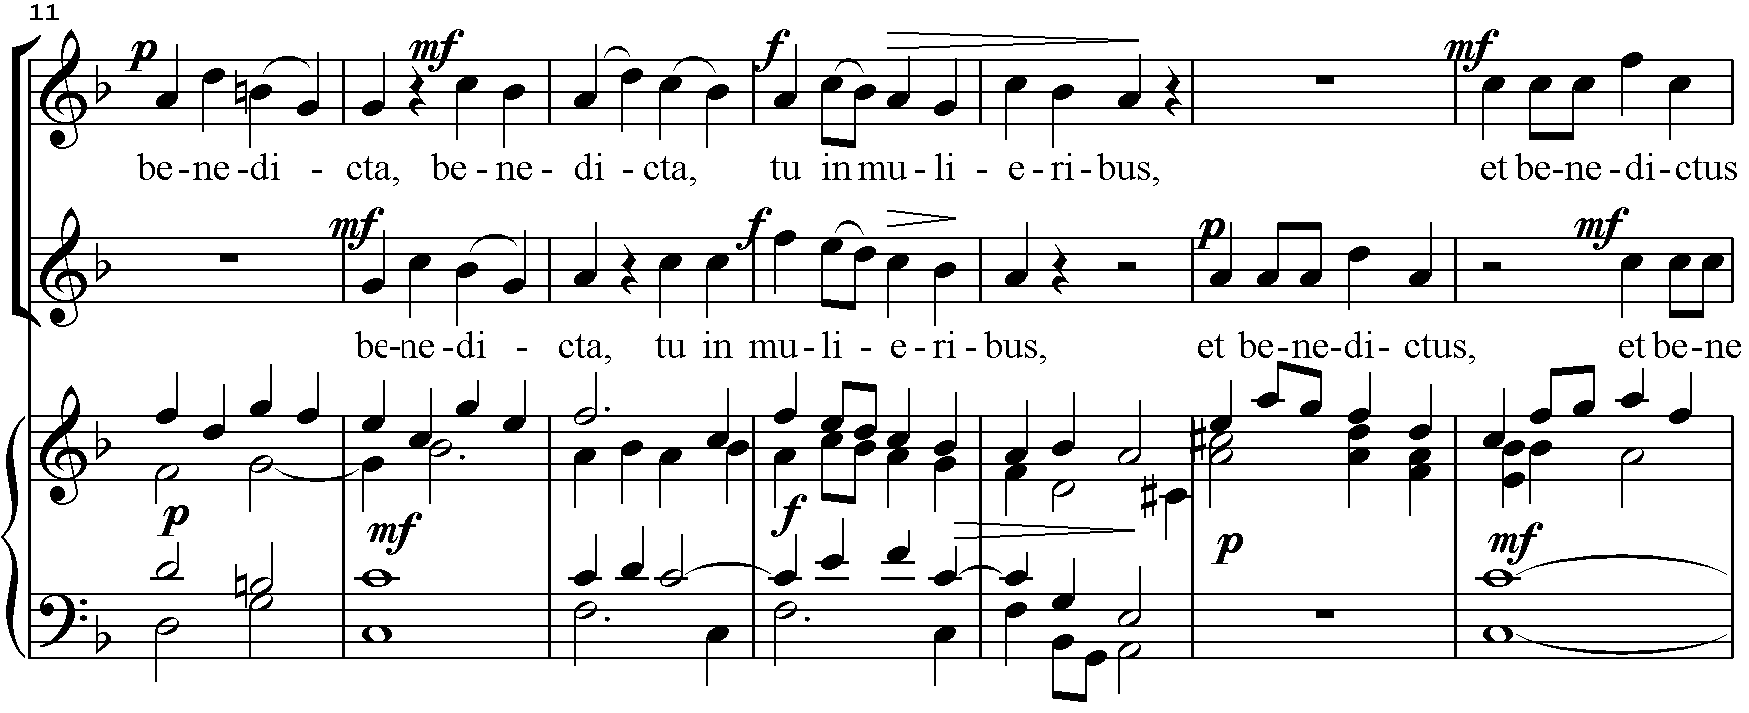
\includegraphics[width=11.382cm,height=4.658cm]{zulassungsarbeit-img/zulassungsarbeit-img095.png}

Op. 4: Ave Maria F-Dur op. 4, Takt 11 –
17, Ober-, Unterstimme und Orgel\\
\end{supertabular}
\end{center}
Eine noch kunstvollere polyphone Satztechnik als die Imitation setzt
Högn im Credo, in den „Hosanna“-Vertonungen des Sanctus und Benedictus
und, wie auf der Abbildung unten zu sehen ist, zu Beginn des Benedictus
der „Laurentius“-Messe C-Dur op. 14 ein: das Fugato.

\begin{center}
\tablefirsthead{}
\tablehead{}
\tabletail{}
\tablelasttail{}
\begin{supertabular}{m{11.948cm}}
  [Warning: Image ignored] % Unhandled or unsupported graphics:
%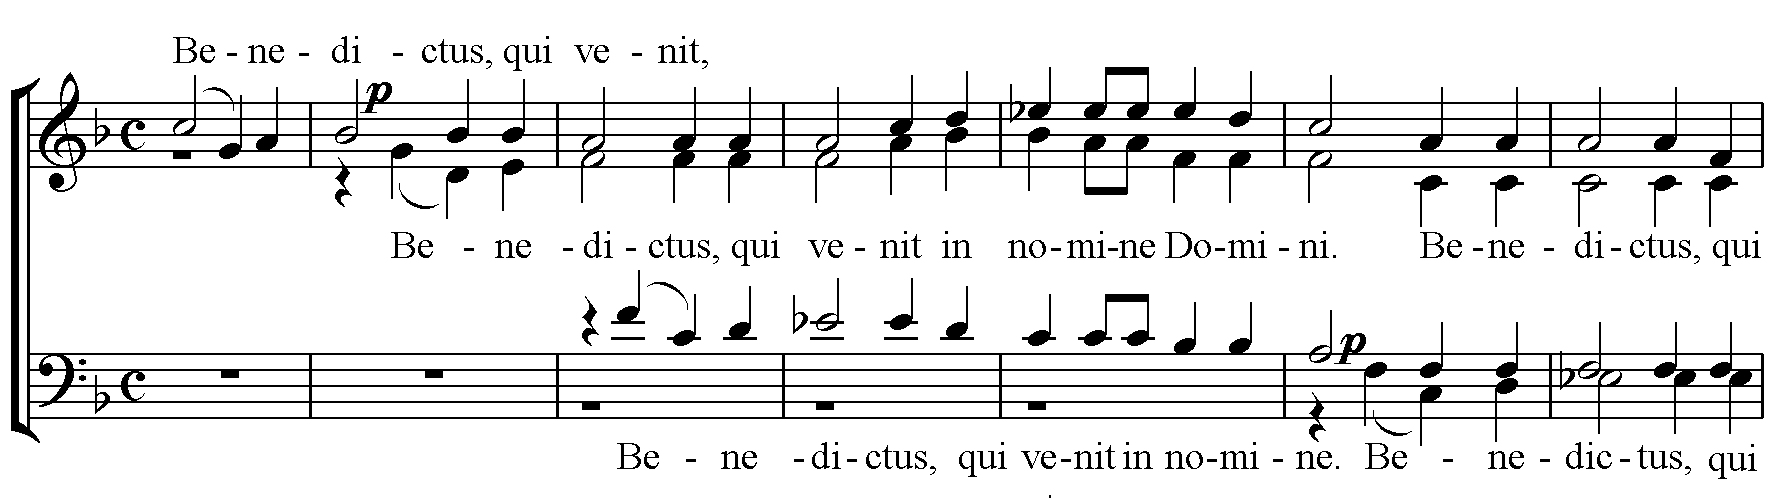
\includegraphics[width=11.765cm,height=3.267cm]{zulassungsarbeit-img/zulassungsarbeit-img096.png}

„Laurentius“-Messe C-Dur op. 14,
Benedictus, Takt 1 – 7, Chor und Orgel\\
\end{supertabular}
\end{center}
Die 11 Veni creator Spiritus op. 15, die 8 Adjuva nos op. 15 und das
Cäcilienlied op. 12 weisen zwar überwiegend eine homophone Satzstruktur
auf, - nur gelegentlich kann eine Imitation zwischen den Stimmpaaren
Sopran-Alt und Tenor-Bass beobachtet werden - doch haben diese Stücke
mit den polyphon gesetzten Kompositionen dieser frühen Schaffensperiode
eine einfache Harmonik gemeinsam und lassen sich deshalb von den Werken
der mittleren, harmonisch weitaus farbigeren Phase deutlich
unterscheiden.

\subparagraph{Mittlere Phase (op. 16 – 50)}
Stilistisch stellt der Übergang von op. 15 zu op. 16 einen Quantensprung
dar und rechtfertigt den Phasenübergang von einem auf das andere Werk.
Ganz unerwartet zeigt sich Högn stilistisch mit der „Mater-Dei“-Messe
F-Dur op. 16, was den Einsatz von Chromatik und erweiterter Harmonik
anbelangt, in einem komplett neuem Gewand.

\begin{center}
\tablefirsthead{}
\tablehead{}
\tabletail{}
\tablelasttail{}
\begin{supertabular}{m{12.027cm}}
  [Warning: Image ignored] % Unhandled or unsupported graphics:
%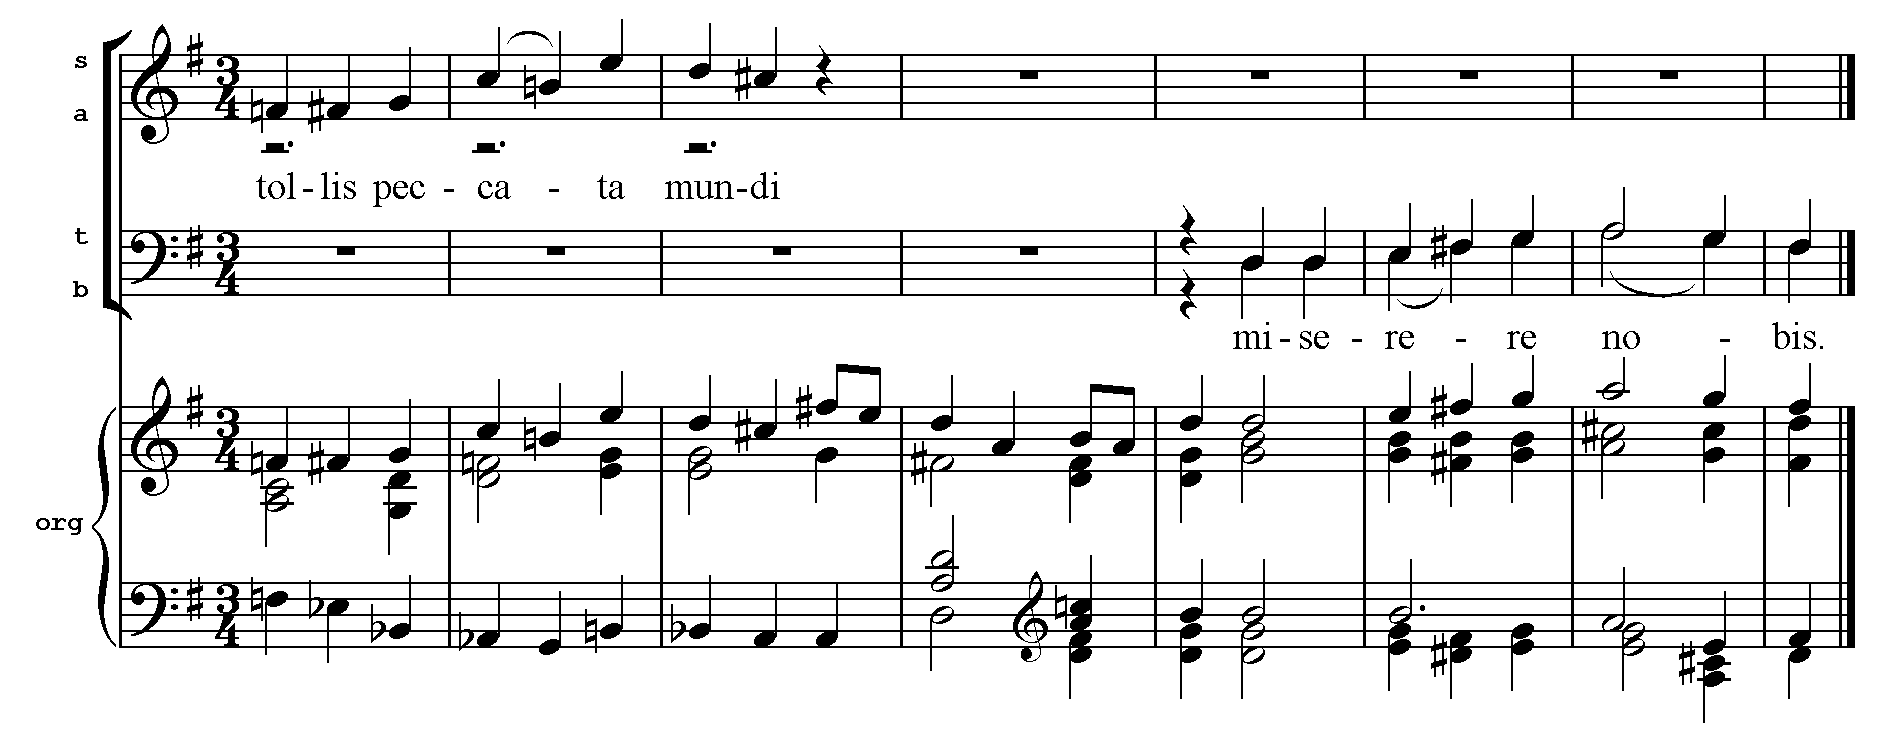
\includegraphics[width=11.845cm,height=4.9cm]{zulassungsarbeit-img/zulassungsarbeit-img097.png}

\label{bkm:Ref99946240}
„Mater-Dei“-Messe F-Dur op. 16, Gloria, Takt  33 – 40, Chor und Orgel\\
\end{supertabular}
\end{center}
Obwohl beide Werke - nach dem Opuszahlen zu urteilen - kurz nacheinander
komponiert wurden, könnte der stilistische Unterschied zwischen der
„Laurentius“-Messe, in der überwiegend Dreiklänge der Grundtonart
verwendet werden, und der „Mater-Dei“-Messe, in der auch abrupte
Ausweichungen in von der Grundtonart weit entfernte Tonarten und
komplexe Vorhaltsbildungen auftreten, kaum größer sein. Ein weiteres
Stilelement tritt mit der „Mater-Dei“-Messe zum ersten Mal und dann
gleich in geballter Form auf. Vier der sechs Messteile stehen in Moll.
Mit Ausnahme des Agnus Deis der „Josephi“-Messe kommt dieses in Högns
ansonsten „Dur-lastigem“ Werk sehr exotisch wirkende Tongeschlecht
weder in der frühen noch in der späten Phase vor. Da Högn ab op. 16 vor
allem klanglich neue Wege beschreitet, war das „Moll“ in dieser Phase
offenbar ein willkommenes Mittel zur Bereicherung der Klanglichkeit.
Das Libera e-moll op. 50 ist die letzte Komposition, die in Moll steht,
und liefert deshalb einen Grund an dieser Opuszahl den Übergang zur
späten Phase fest zu machen. Einher mit den Versuchen einer
harmonischen Klangerweiterung geht die Gewichtsverlagerung von den
figurierten imitatorischen Sätzen der Frühphase zum vorwiegend in der
mittleren Phase anzutreffenden homophonen Satz.

\begin{center}
\tablefirsthead{}
\tablehead{}
\tabletail{}
\tablelasttail{}
\begin{supertabular}{m{11.78cm}}
  [Warning: Image ignored] % Unhandled or unsupported graphics:
%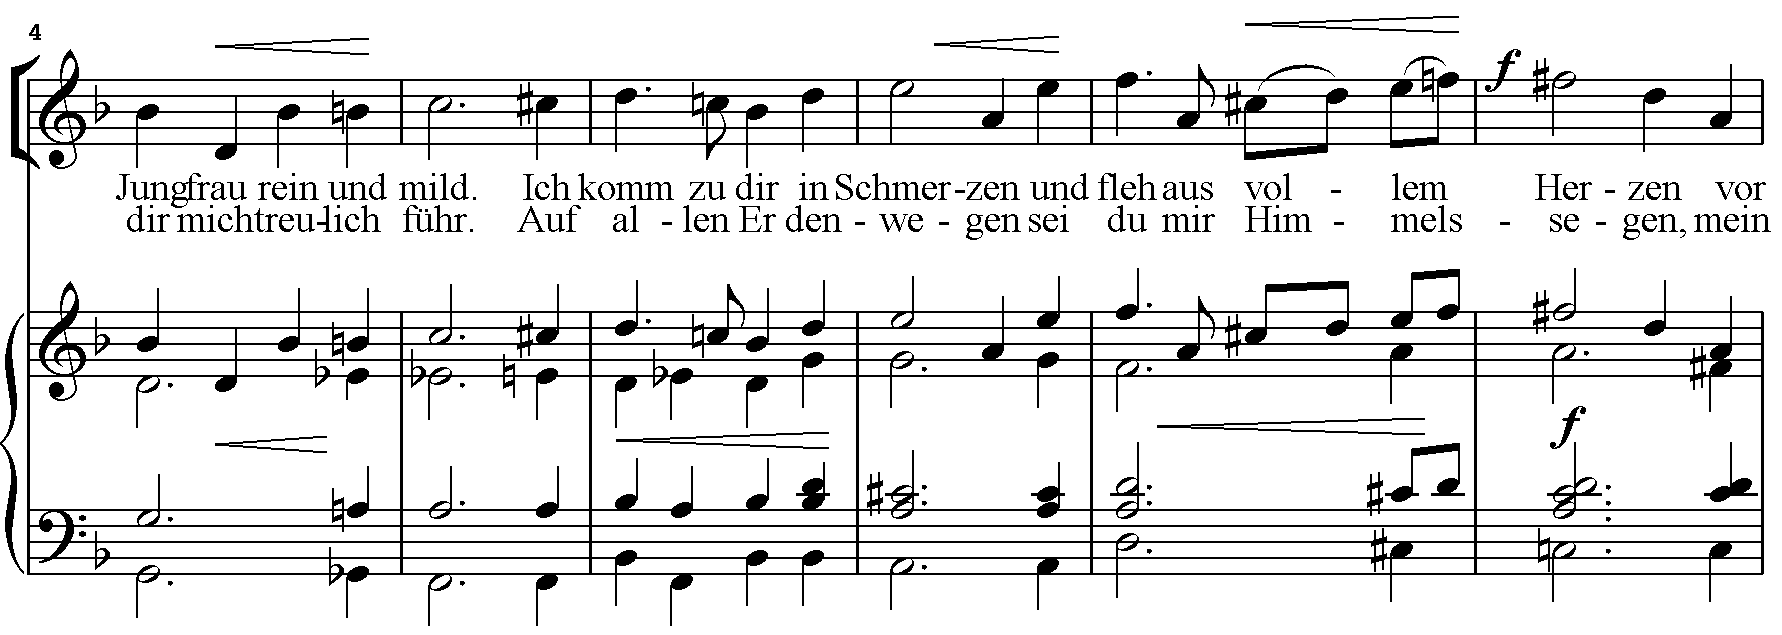
\includegraphics[width=11.598cm,height=4.133cm]{zulassungsarbeit-img/zulassungsarbeit-img098.png}

\label{bkm:Ref99946259}Marienlied Nr. 3
F-Dur op. 22, Takt 4 – 9, Sopran-Solo und Orgel\\
\end{supertabular}
\end{center}
Auch innerhalb der mittleren Schaffensperiode lässt sich eine
stilistische Weiterentwicklung feststellen. In den ersten Werken der
mittleren Phase gibt es Kompositionen mit teilweise abrupten
Modulationen und sehr chromatisch durchsetzten Gesangsstimmen, wie zum
Beispiel im Gloria von Takt 33 – 40 der „Mater-Dei“-Messe (Abb. 95)
oder im Takt 4 – 9 des Marienlieds Nr. 3 F-Dur op. 22 (Abb. 96)
festzustellen ist. Spätere Kompositionen weisen zwar immer noch eine
farbige Harmonik auf, doch wirkt diese keinesfalls mehr so scharf wie
zu Beginn der Phase, sondern ist eingebettet in einem lieblichen und
weichen Tonfall. Das Tantum ergo Nr. 2 F-Dur op. 32 ist ein Beispiel
dafür.

\begin{center}
\tablefirsthead{}
\tablehead{}
\tabletail{}
\tablelasttail{}
\begin{supertabular}{m{8.399cm}}
{\centering   [Warning: Image ignored]
% Unhandled or unsupported graphics:
%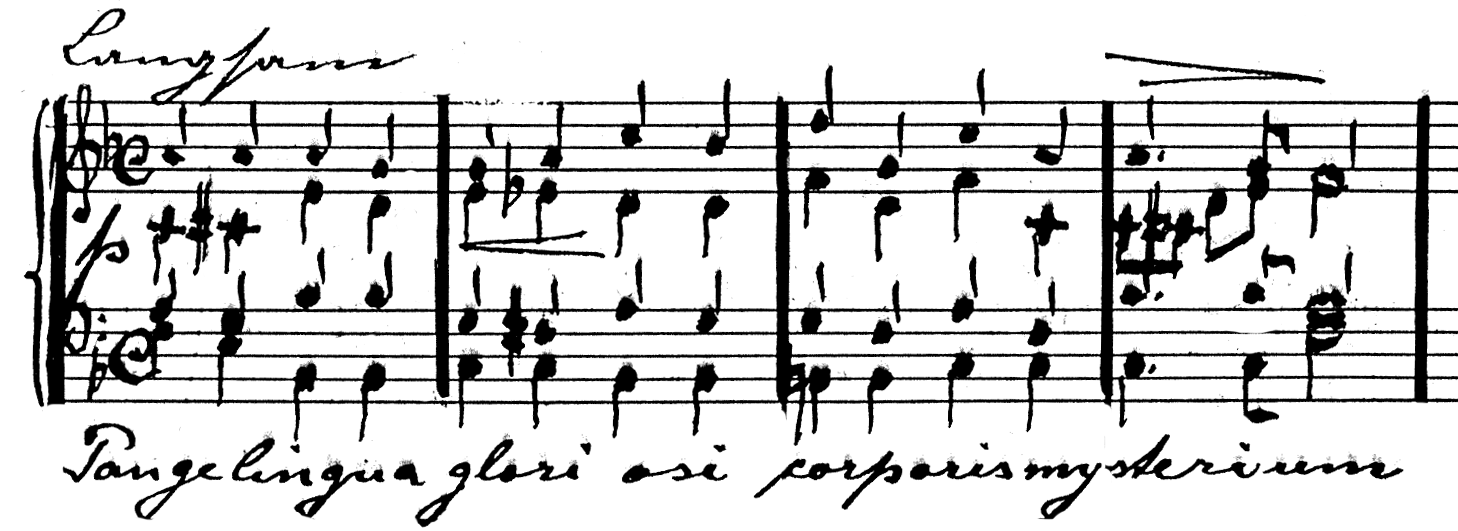
\includegraphics[width=8.216cm,height=3.006cm]{zulassungsarbeit-img/zulassungsarbeit-img099.png}
 \par}
Tantum ergo Nr. 2 F-Dur op. 32, Takt 1
– 4, Chor\\
\end{supertabular}
\end{center}
\subparagraph[Späte Phase (op. 51 – 63)]{Späte Phase (op. 51 – 63)}
Eine Grenze zwischen der mittleren Phase und späten Phase lässt sich
nach op. 50 ziehen, da das Libera e-moll op. 50 wie bereits erwähnt die
letzte in Moll stehende Komposition in Högns musikalischen Schaffen
darstellt. Auch das Hinzutreten eines neuen stilistischen Elements
rechtfertigt eine Unterteilung in eine weitere Phase. Anklänge aus der
bayerischen Volksmusik mischen sich unter Högns Tonsprache. Ganz
deutlich zeigen den folkloristischen Einfluss Passagen, die Ruhe und
Gelassenheit vermitteln, aus dem Ecce sacerdos F-Dur op. 57 (Takt 23 –
36) und der „Josephi”-Messe F-Dur op. 62 (Gloria Takt 31 – 52, Credo
Takt 45 – 56 Takt 91 – 103, Sanctus 11 – 14, komplettes Benedictus).

\begin{center}
\tablefirsthead{}
\tablehead{}
\tabletail{}
\tablelasttail{}
\begin{supertabular}{m{12.034cm}}
  [Warning: Image ignored] % Unhandled or unsupported graphics:
%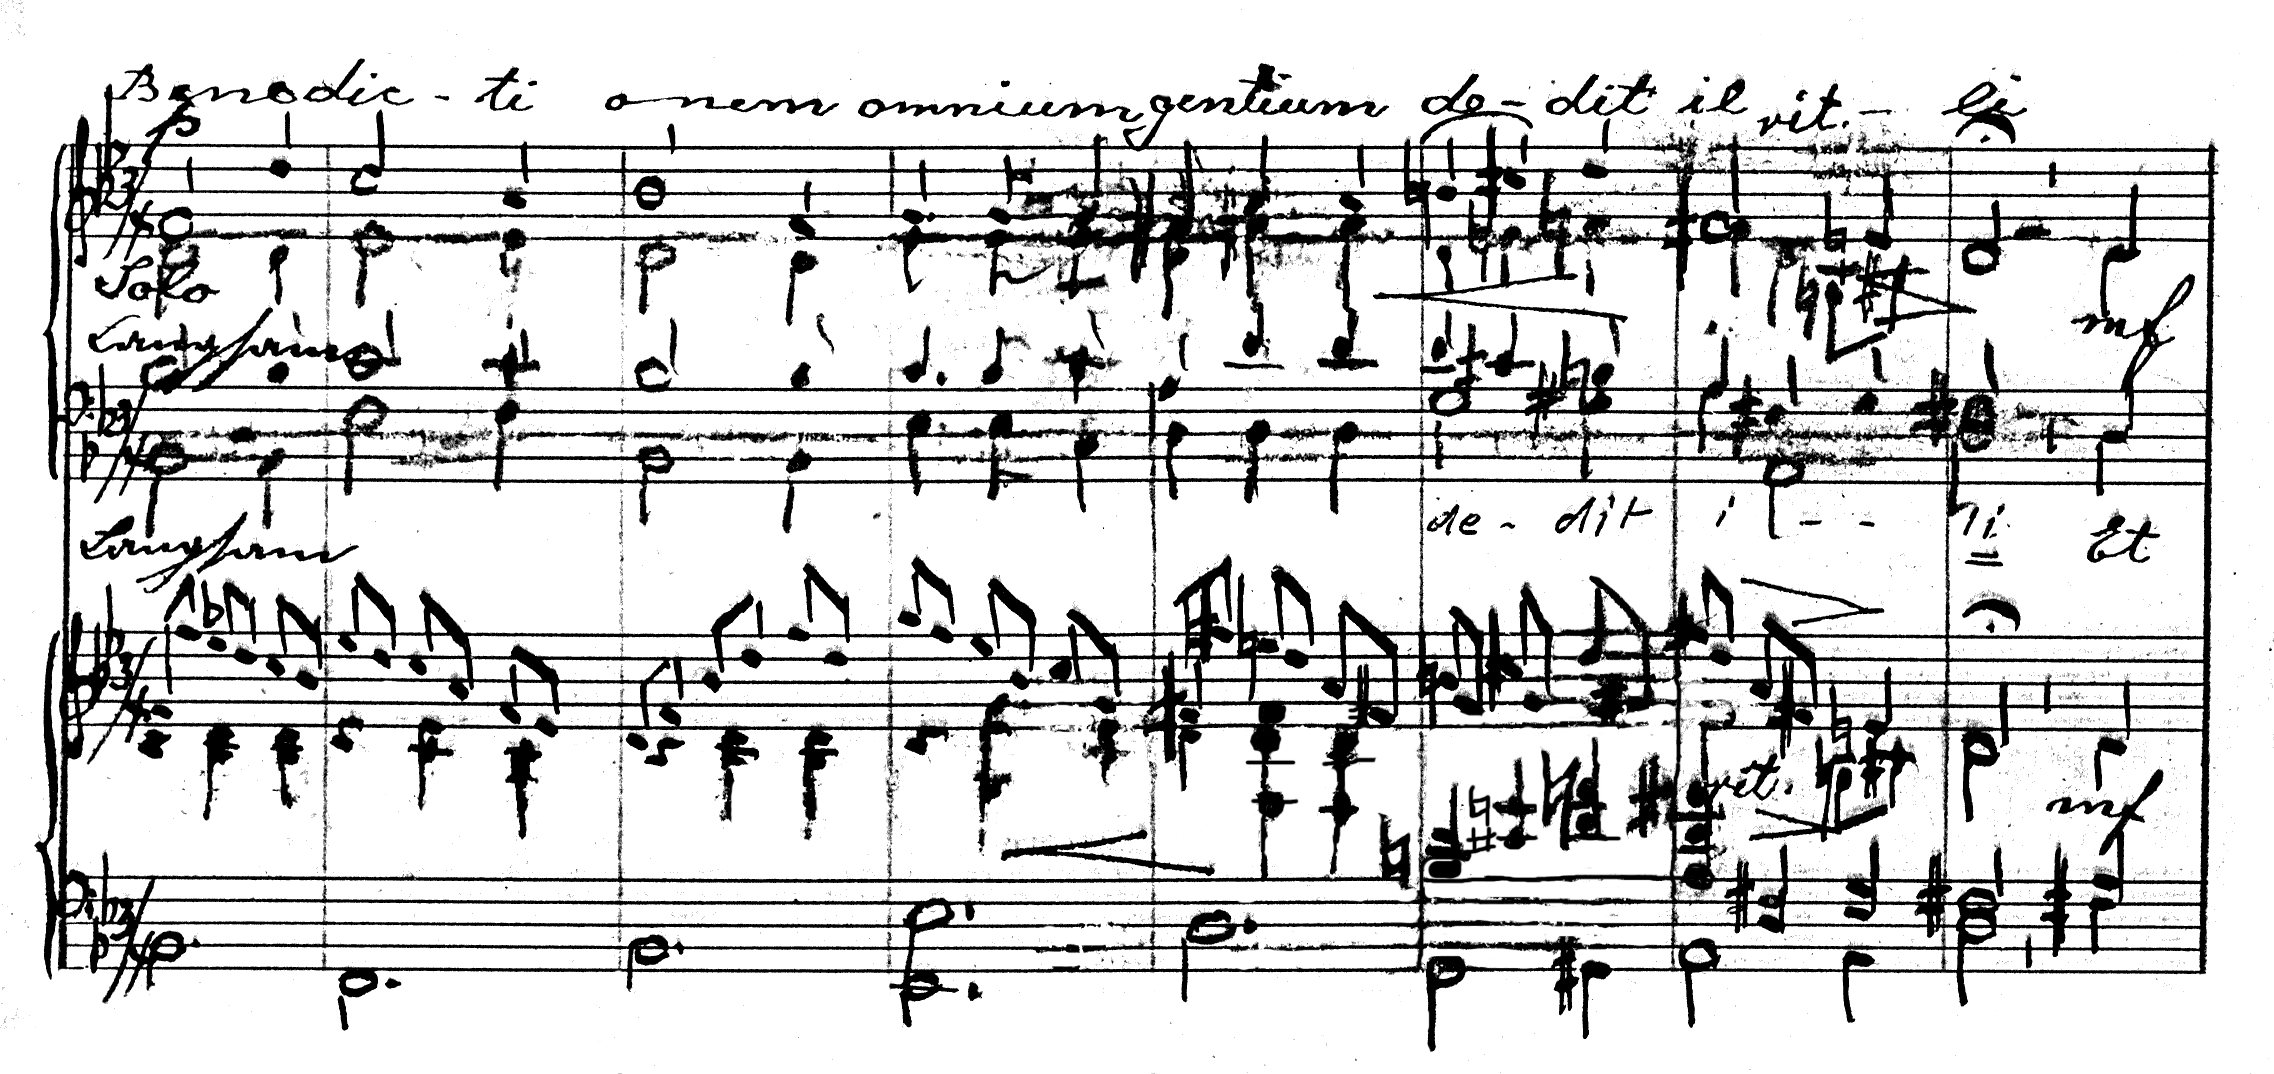
\includegraphics[width=11.852cm,height=5.583cm]{zulassungsarbeit-img/zulassungsarbeit-img100.png}

\label{bkm:Ref99948828}Ecce sacerdos
F-Dur op. 57, Takt 23 – 30, Chor und Orgel\\
\end{supertabular}
\end{center}
Die Orgel gibt an diesen Stellen ihr „colla-parte“-Spiel auf und
begleitet den Chor \newline
oder die Solostimmen mit tonikalen oder dominantischen Harmonien unter
einer \newline
Oberstimme in fließenden Achteln. Wenn in der Orgelstimme zusätzlich zu
der \newline
Oberstimmenbewegung noch eine in Terzen oder Sexten geführte zweite
Stimme hinzutritt, wie im Credo der „Josephi”-Messe von Takt 45 – 51
(Abb. 99), oder als weiteres Begleitungselement nachschlagende Akkorde
gesetzt werden, wie im Ecce sacerdos von Takt 23 – 30 (Abb. 98), drängt
sich eine Assoziation mit bayerischer Volksmusik geradezu auf.

\begin{center}
\tablefirsthead{}
\tablehead{}
\tabletail{}
\tablelasttail{}
\begin{supertabular}{m{11.729cm}}
  [Warning: Image ignored] % Unhandled or unsupported graphics:
%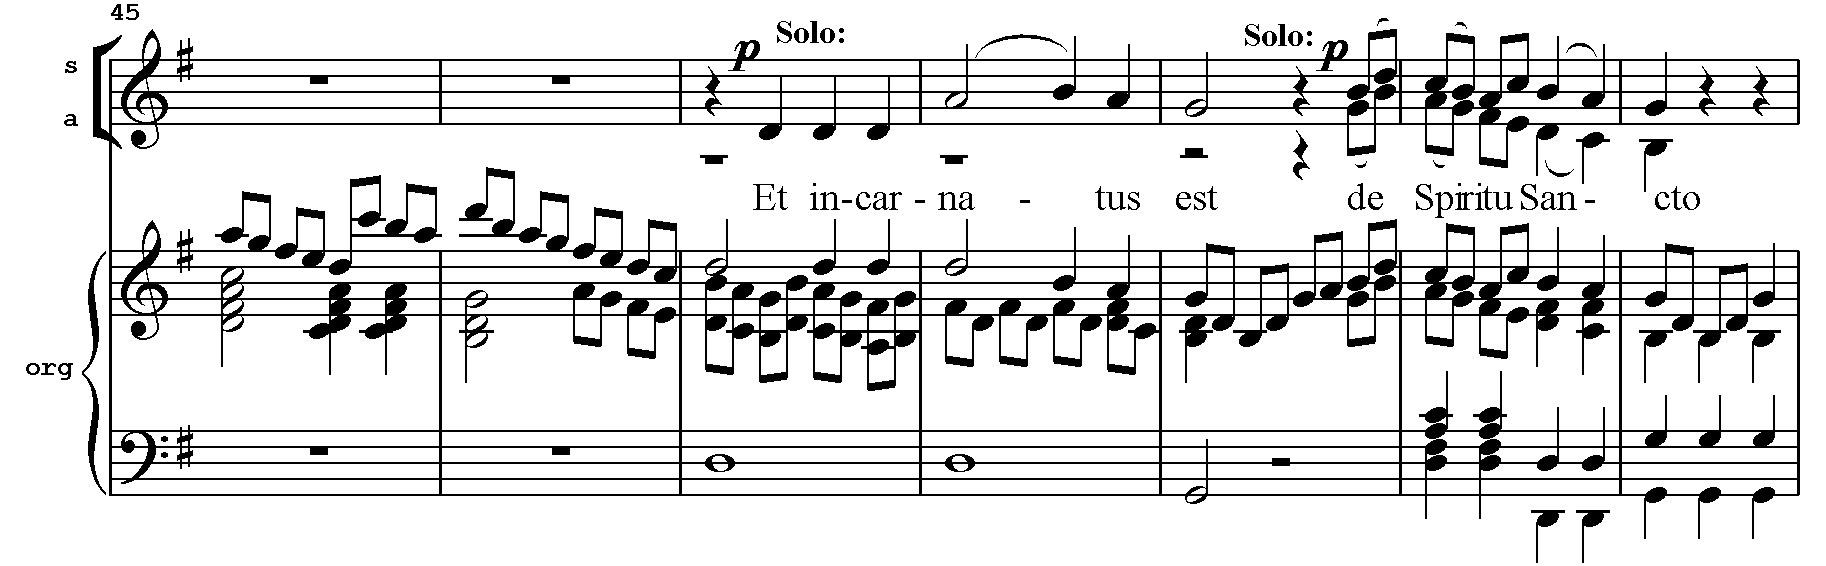
\includegraphics[width=11.546cm,height=3.787cm]{zulassungsarbeit-img/zulassungsarbeit-img101.png}

\label{bkm:Ref99948855}„Josephi”-Messe
F-Dur op. 62, Credo, Takt 45 – 51, Orgel, Sopran- und Alt-Solo\\
\end{supertabular}
\end{center}
Die zwar immer noch harmonisch farbige, aber im Gegensatz zu den
früheren Stücken der mittleren Phase lieblich und schlicht wirkende
Tonsprache verleihen den Kompositionen der letzten Phase auch über
diese Einschübe hinaus einen volkstümlichen Charakter.

Diese folkloristischen Anklänge stellen das einzige Stilelement dar, das
Högn nicht aus ihm zugänglichen Kirchenmusiken, sondern aus der
weltlichen Volksmusik oder volkstümlichen Musik übernommen hat. Wie
sein angebliches Lieblingslied „Grün ist die Heide“ \footnote{ Dokument
Nr. 49, Zeitungsartikel aus Viechtacher Bayerwald-Bote, 5.8.1958}
verrät, war die volkstümliche Musik Högns favorisierte Musikrichtung.
Die Integration dieses Elements aus einem außerkirchenmusikalischen
Stil in seine geistlichen Kompositionen kann als Eigenleistung Högns
angesehen werden. Es ist vor allem diesem folkloristischen Stilelement
in Högns spätem Werk zuzuschreiben, dass an Kompositionen aus Högns
später Phase ein unverwechselbarer Personalstil festgestellt werden
kann.